\section{Ausgangszustand}
Zum Beginn dieser Arbeit wurde bereits in meiner vorangegangen Tätigkeit bei der Hoffmann Group auf Basis des NRF52840-Dongle prototypisch eine Anwendung implementiert, die auf das Bluetooth Modul der Hoffmann Group aufbaut und in der Lage ist, sich selbstständig mit mehreren Drehmomentschlüsseln zu verbinden. Sie stellt die Messergebnisse bereits über einen virtuellen COM-Port im MUX50 bzw. DMX16 Protokoll zur Verfügung und die zu verbindenden Geräte sind über eine \ac{CSV}-Datei, die über \ac{MSC} dem Nutzer zur Verfügung gestellt wird, konfigurierbar.

\subsection{Aufbau}
Die Anwendung nutzt das Bluetooth Modul der Hoffmann Group. Es stellt dabei die Anwendungsschicht des \ac{BLE}-Stack da und abstrahiert somit die \ac{BLE} spezifischen Aufrufe zum Softdevice. Es wird in allen \ac{HCT}-Werkzeugen eingesetzt, wo es eine Vermittlerfunktion zwischen dem eigentlichen Gerätechip und dem Softdevice übernimmt, dabei kann es sowohl in peripheral und central Rolle agieren. Es führt den Verbindungsprozess zu Computern und \ac{HCT}-Geräten durch. Als Softdevice wird das S140 von Nordic Semiconductor in der Version 7.2.0 verwendet. \\
Auf diesem Basisprojekt aufbauend befindet sich die \ac{USB}-Dongle App. Im Gegensatz zu den \ac{HCT}-Werkzeugen sitzt die gesamte Anwendung ebenfalls auf dem Chip des Softdevice und muss sich die Chipressourcen mit ihm teilen. Die Funktionalität, die in dem File usb\_dongle\_app.c gekapselt ist, ist dafür zuständig das Konfigurationsfile einzulesen und die zugehörigen Daten während der Laufzeit zu halten. Dabei handelt sich es um die zu verbindenden \ac{HCT}-Gerät, welche in einer gleichnamigen Struktur mit Name, Seriennummer und einer Kanalzuweisung gespeichert werden. Die Kanalzuweisung wird für das MUX50 bzw. DMX16 Protokoll benötigt. Werden die Geräte dann verbunden, muss weiterhin der Verbindungszustand, sowie das Connection-Handle gespeichert werden. Des weiteren sammelt es die Messdaten auf, die vom Central Device von den \ac{HCT}-Geräten im Interrupt-Kontext empfangen werden und reiht die Daten, die von Interesse sind, in eine \ac{FIFO} Nachrichtenqueue ein. Diese werden später aus dem Kontext der Main-Loop heraus, in das MUX50 bzw. DMX16 Protokoll umgewandelt und über den virtuellen COM-Port verschickt. Ebenfalls in der Funktionalität des usb\_dongle\_app.c Files und aus dem Kontext des Main-Loop heraus, werden die Befehle des MUX50 Protokolls, welche über dem virtuellen COM-Port empfangen wurden, verarbeitet.\\
In dem File usbd\_msc\_cdc\_composite.c werden \ac{USB} spezifischen Aufrufe gekapselt. Hier wird das \ac{MSC} und der virtuelle COM-Port (CDC) initialisiert und konfiguriert. Der Code wurde nur mit kleinen Änderungen aus den Beispielen des NRF\_SDKs übernommen, weswegen nicht weiter auf die Implementierung eingegangen wird.\\
Da es keine Unterstützung seitens der NRF Bibliothek für den internen Flash als Speichermedium für das \ac{MSC} gibt, musste der Treiber block\_device\_ram.c angepasst werden. Er wurde als block\_dev\_fStorage.c in das Projekt gezogen und ruft die Funktionen des Files fStorage.c auf, welches die Schreibbefehle im Interrupt-Kontext ebenfalls in eine \ac{FIFO} Nachrichtenqueue einreiht. Das ist nötig, da für die korrekte Ausführung auf Interrupts des Flash Memory gewartet werden muss, welche nur im Kontext der Main-Loop korrekt empfangen werden. Zudem wird dort Flash Memory spezifische Logik abstrahiert. So muss eine Flash Page erst "erased" werden, bevor sie geschrieben werden kann und die Block Logik des \ac{MSC} wird auf die Flash Page Logik des Speichers übertragen.

\begin{figure}[H] 
	\centering
	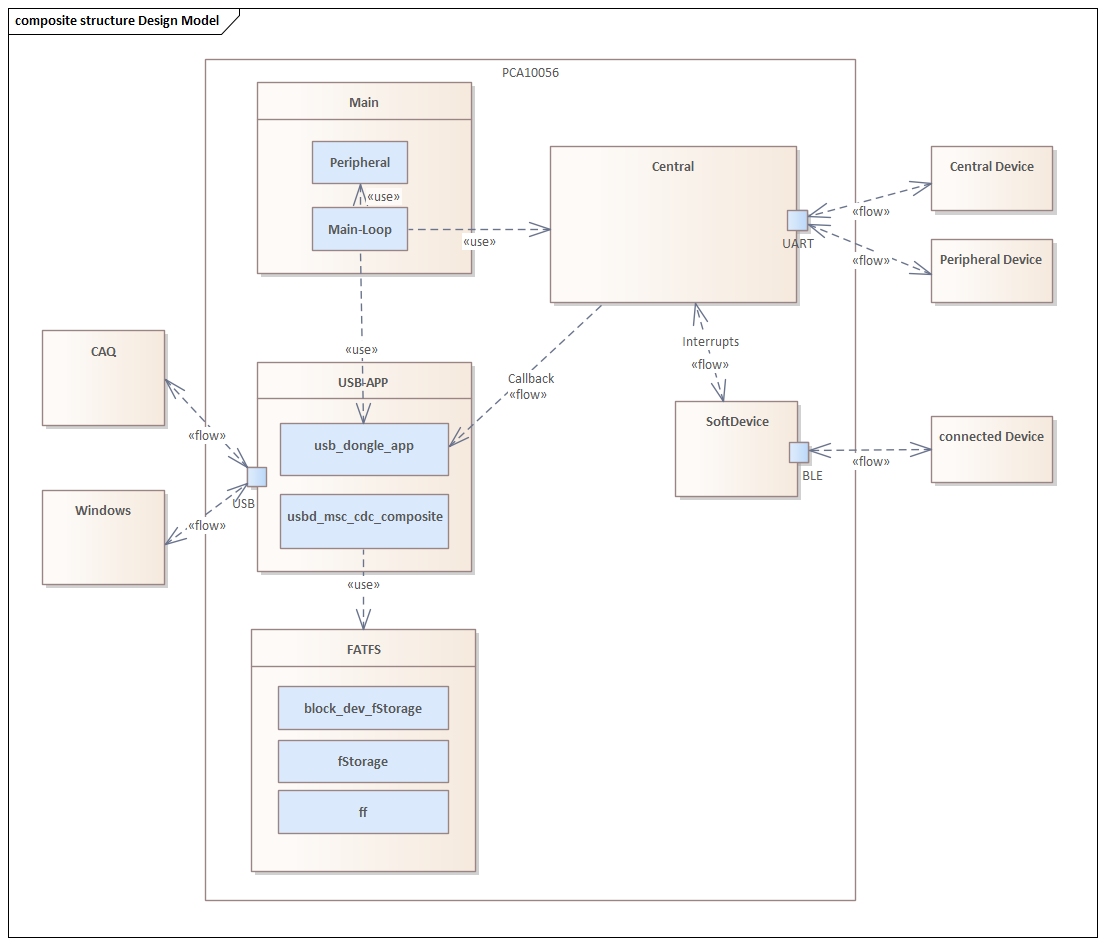
\includegraphics[width=\textwidth]{figures/Design_Model.png}
	\caption{Aufbau \ac{USB}-Dongle App}
\end{figure}


\subsection{Erweiterungen für Fußschalter}
Für den Fußschalter muss die bestehende Software wie folgt erweitert werden. Die Peripherie des Fußschalter muss eingebunden werden. Diese umfasst den Schalter der durch den Anwender betätigt werden kann, eine LED-Leuchte und den Akku des Fußschalters. In Hinblick auf den Akku muss eine Energiemanagement geschaffen werden, um dessen Kapazität zu schonen. Zudem sollen die Messmodi \ac{USB}-\ac{HID}, \ac{USB}-\ac{HID}-Single-Character, \ac{BLE}-\ac{HID} und \ac{BLE}-Windows-App geschaffen werden. Diese sollen sich neben den \ac{HID}-spezifischen Konfigurationen in einer eigenen Datei befinden. Des Weiteren müssen die Schreibbefehle des \ac{MSC} optimiert werden, da sie nur sehr langsam und fehlerbehaftet abgearbeitet werden. Die Änderungen an der Konfiguration der Anwendung wird außerdem erst übernommen, wenn der Dongle abgezogen und wieder angesteckt wird, also die Anwendung neugestartet wird. Beim Fußschalter sollen Änderungen an den Konfigurationsfiles detektiert werden und die Anwendung programmatisch neugestartet werden, auch weil durch den Akku die Anwendung durch den Nutzer nicht direkt neugestartet werden kann. Es müssen außerdem die Messuhren bzw. Messschieber eingebunden werden. Zusätzlich soll die Anwendung weiterhin auch als Dongle erhältlich gemacht werden und die Implementierung muss in Hinblick auf diese Hardwarunterschiede durchgeführt werden.